\documentclass[11pt]{article}

\usepackage{fullpage}
\usepackage{graphicx}
\graphicspath{ {./images/} }

\begin{document}

\title{ARM Project Final Report}
\author{Group 40 - Amelia Khavari, Ibrahim Munir-Zubair, Luke Texon, Umer Hasan}

\maketitle

\section{Assembler}
We approached the assembler in a similar way to the emulator, splitting the work into smaller submodules, namely the main module where the assembly is done, a module for parsing operands, miscellaneous utility functions, a mnemonic parser for changing strings into enums and a hash map module for the symbol table. Required functions were declared within header files before implementation, albeit many declarations needed later revision.

We also made use of, and updated, the binary operations module from emulator, as we were still working with binary strings, and the binary file I/O module, for writing to binary files.     

We opted for a two-pass implementation of assembly to avoid memory complications. The design was easier to implement and more modular. Furthermore, there was no significant advantage to a one pass assembly. 
The program reads through the input file once, building up the symbol table and storing the assembly instruction lines in an array. The output binary file produced contains the converted instructions as well as contents of the reserve memory too. To avoid the continual reallocation of memory or the use of a linked list, a fixed size array is allocated for reserve memory during assembly. Each instruction requires at most one reserve memory location; therefore, we allocated the same amount of memory to the reserve memory as we did the instructions.

After initializing any data structures to be used, the second pass then consists of iterating through the assembly instruction lines in a sequential manner and using an encoding function to assemble each instruction and store it in an instructions array. To do this, it uses regular expressions to find the type of each instruction, then uses tokenisation to parse the instruction to retrieve the required register numbers and flags, and then delegates assembly to the appropriate helper function accordingly. 
The helper functions responsible for producing the binary instructions each return the instruction in the form of a WORD, a user-defined type representing a 32-bit word as in ARM. The single data transfer helper function is additionally passed the address of the instruction as well as next reserve memory location so that the program is able to store any immediate values that are too large for a mov instruction.
The branch helper function is also passed the address of the instruction as well as the symbol table, so it can calculate the branch offset.
There are three helper functions called from the assembly function for data processing: for move operations, logical test operations and general data processing operations. Both of these functions call a third helper function with appropriate parameters, which completes the conversion into machine code.

All functions in the program have been carefully designed so they are self-contained, taking in their required parameters as either pointers or values, de-referencing pointers as appropriate and returning their result values.

Each member was assigned to implement either a number of helper functions or an entire module, depending on the difficulty. Group members helped each other debug and test code to ensure the code style was up to scratch and to catch any logical mishaps in the algorithms used. Understanding the overall workings of all parts of the program was important in ensuring that each group members individual contribution complemented the existing code and avoided code duplication. In some cases, we worked as a whole group to code or debug some aspects of the program. The majority of the design decisions were made as a group, and the implementation of more complicated functions was carried out in person so that everyone was in the loop. 

\section{Extension}
\subsection{Description}
Our extension is focussed on the statistical modelling and prediction of equity prices. We use a neural network with tuned inputs and an expected outcome to then predict the next day price of the specific instrument in question. We decided to focus on heavily traded asset classes such as S\&P500 stocks and foreign exchange. These are not too volatile hence are a good idea for a neural network to start training on. Neural networks are being increasingly used in forecasting time series due to their new unique method of technical analysis. When combined with traditional technical metrics, this could potentially lead to some alpha generation. Alpha gauges the performance of an investment against a benchmark market index. 

The idea for the extension was extremely ambitious as it takes teams of several talented quantitative researchers years to create a significantly profitable strategy that outperforms the market in all scenarios. We believe that a good start was made on the attempt to implement such a strategy in C. The project was applicable to the C language as extremely fast execution is required for the task and professionals are getting down to the assembly and memory management levels to give their strategy the extra edge. However, one point to consider is that a strategy is typically first implemented in a higher level language such as C++ before being translated to C. We did not have this luxury so we focused on creating a simple backtest to train and test the neural network. This was done by importing a 5 year CSV using a python script on daily trade data. 

A backtest isn't sufficient to predict live stock prices but gives a good idea of whether the crude strategy is something which should be pursued and refined further. Typically a neural network accuracy of anywhere from 55\% to 70\% is industry standard. This is because it is noticeably better than a 50/50 and going past a 70\% accuracy is almost certainly a sign of overfitting the model to the data. 

The end result was to use a neural network to predict the next day's price using 6 inputs calculated from previous days prices and volumes. An example where it could be used would be to combine the model with several other models to create a comprehensive technical trading strategy. Since the financial markets are essentially a time-series problem at heart, the model would be applicable to other situations where some forecasting is required. 

\begin{figure}[h]
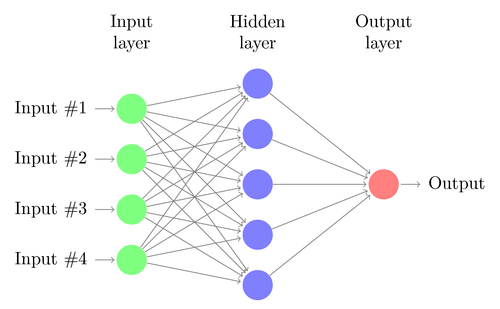
\includegraphics[scale=0.8]{neural-network}
\caption{Example diagram of a neural network$^1$}
\end{figure}

\subsection{Design}
In order to access the data, a python script was used to import CSVs into a folder. The C program then imports the CSV and runs the pre-processing functions on the data to output a 2D-array containing the 6 neural network inputs and an array of prices. The train test data was split 70/30.

The inputs were specifically chosen as commonly used momentum-based technical indicators which would aim to train the neural network on the direction the specific stock price would go towards. There were 6 inputs which were created using the functions in the pre-processing.c file. 

The first input was the log of the return with the return being a specific day's price divided by the day before's price. The second input was the volume of shares traded on the day. The third input was an exponential moving average (EMA) of the log return. An EMA takes into account a specific time period of days prior to the current day and calculates an average with exponentially more weight on the prices of the more recent days. The fourth input was the relative strength index (RSI) which indicates whether a specific asset is over-bought or over-sold and signifies which lifecycle the momentum is in. The fifth input was a moving average convergence divergence (MACD), this is calculated by subtracting a longer time period EMA from a shorter time period EMA. This signifies a specific trend that is taking over in the short term. This, in turn, signifies a momentum change. The last input was the rate of change of the stock price. This is quite similar to the log of return and may not add as much value as the rest of the indicators. However, it was important to add another input directly linked to short term price changes to emphasise the importance of the short term trend in price.

The weights are initialized randomly. As the neural network trains, it learns by refining the link weights. This process is guided by the error, which is the difference between the desired and actual output. 

The weights are used in 2 ways, firstly for propagating signals forwards from the input to the output layers. Secondly, to propagate the error back from the output back into the network. This process is used to train the network and is known as backpropagation. 

The following files are contained in the src/neuralNet/ directory.

\begin{itemize}
    \item \textbf{layer.c, layer.h} contains implementation of a single neural network layer 
    \item \textbf{loader.c loader.h} contains utility functions for training and implementing neural network
    \item \textbf{neuralNet.c neuralNet.h} contains primary functions memory management of neural network
    \item \textbf{preprocessing.c preprocessing.h} contains functions for importing the data and pre-processing neural network inputs
    \item \textbf{trainNeuralNet.c} main file for training and running the program
\end{itemize}

\subsection{Challenges}
The main challenge was that the group as a whole had little experience in the use and implementation of neural networks. 
Therefore, we used this as a learning experience and an introduction to neural networks. 
Much of the time implementing the extension involved understanding how they work.

We had to adapt the neural network implementation as it originally only accommodated for values between 0 and 1.
To allow for any scalar value to be used, the inputs have to be normalised to values in this range
and the resulting output must be denormalised using an inverse process to the normalisation.

We were unsure about what hyperparameters to use without preliminary calculations. This included the learning rate, the number of epochs and the ratio of training to testing data. These values could drastically change the result of training; too few epochs could cause underfitting. 
In the end, we opted for 500 epochs, a learning rate of 1 and a ratio of 70:30 for training to testing data.
Another challenge was in the web scraping. Originally, we attempted to write a web scraper in C, however, C is a hardware-level language that is not designed for using web requests and accessing websites. Consequently, we implemented the web scraper in Python.

On several occasions, we encountered memory errors that hindered our progress. These normally occurred due to incorrect array access and were occasionally due to the excessive allocation of the heap. This was due to a new pointer being allocated in a for loop which was unnecessary. 

\subsection{Testing}
The data was split into training and testing data as is common practice in machine learning projects. As for how the implementation was tested, there were test functions created and placed in a separate file for each section of the project. The data pre-processing was an easier section to check as it was mostly to do with file reading. This would clearly be successful if the arrays were populated. The mathematical functions were not complex hence did not need extensive testing. Some sample fake data was made to test and tune parameters on the neural network while the pre-processor was being written. These are included in the test file. 

The testing was not as effective as an extensive testing suite or library, however, it was sufficient given the time and scope of the project. Clearly, in future, we would add more tests for each parameter inputted into the model.

One such result was an accuracy of 40\% for the network training on 3.5 years of Coca-Cola Company stock price data. The error margin was 3\% for the prediction, hence, it is better than random. Typically for a trade to be made a significant upside of greater than 3\% is needed (with trading costs themselves being around 1\% or 2\%). This means our error was not significant. The accuracy suggests the model could be combined with other methods of technical and fundamental analysis to create an overall strategy. 

\begin{figure}
\centering
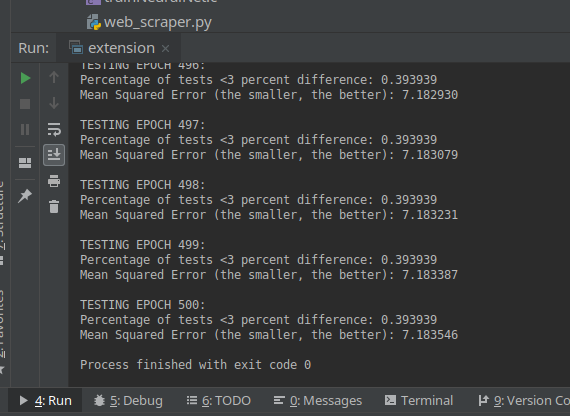
\includegraphics[scale=0.5]{accuracy}
\caption{Screenshot of accuracy}
\end{figure}

\section{Group Reflection}
We communicated efficiently through the use of the VoIP application Discord. 
Discord allows for text messaging, voice calls and, most notably, screen sharing.
Screen sharing allowed us to do pair programming while being in different locations. This helped significantly with debugging as well. 

During discussions, we would organise regular meetings and coding sessions. We thoroughly planned the implementation of emulator and assembler; we prepared header files containing function signatures
for required functions that required implementation. This way, we could assume functions were correct and could program concurrently.
This increased group productivity and 
On the other hand, this only helped to an extent. Many function signatures needed later alterations as the implementation required different parameters and these changes needed to be propagated across the different functions and modules that called it.

\section{Individual Reflections}
\subsection{Amelia's Reflection}
I feel our group has worked together very well as a team. Our team leader made sure to split up the tasks evenly giving everyone the opportunity to contribute and learn. For our extension we considered several ideas, I was particularly keen on building an electric skateboard, however, due to financial constraints this was not feasible so instead, I put forward the idea of building a neural network inspired by one of the past papers. Previous experience in neural networks enabled me to take control during this part of the project. Another team member had significant experience with stock trading resulting in our final idea. This enabled us to work very well as a group delegating subtasks depending on everyone's strengths. I am also proud of the hashmap data type I implemented for the symbol table as part of the assembler. Working on it helped me understand the C language a lot more thoroughly. However, after developing the data type I realised it was unnecessary for this particular project because such few data needs to be stored so an array would be sufficient. Using Git has been an obstacle for me due to handling merge conflicts but this has forced me to get to understand it a lot better.

\subsection{Ibrahim's Reflection}
This group project was an important learning experience for me, having only ever worked independantly on programming projects before. Due to the absence of a group member for the first part, I took a larger responsiblity in planning the program structure and building up the codebase. Initially, I worked on I/O and the main function, which allowed us to test the more detailed parts of the program as they were built up. As I did not take responsibility for the longer sections, my role following this largely consisted of checking code for correctness and style, debugging, planning, and fixing integration errors. Due to my somewhat perfectionist nature, I found myself feeling critical of some solutions presented by others, and wanting to take a greater role in writing the code. However, this being a group project, I took a step back and ensured that this did not affect our teamwork or outcome. The project manager did well in delegating tasks depending on each group member's skills. In future projects, it would be wise to plan properly before starting, as I feel this was a weakness of ours and slowed down development noticably as we approached the difficult sections. We also could have used git more effectively to help manage group development.

\subsection{Luke's Reflection}
I think the group project went well and I had a suitable role in the group.
I like to believe my coding and debugging skills were valuable to the team.
During this project, I realised that my speed of programming could be improved by a lot,
normally coding slower than the rest of my teammates. I accommodated for this
with my debugging skills and by thoroughly inspecting the code.
My literary skills also found a place in contributing to the report.
In my next team, I would like to continue planning as we did in this project.
Although, I would like to plan objectives and actions more thoroughly in future so that
any unforeseen circumstances are covered and their negative effects on group productivity are minimised. The way we divided the work between members is another
method that I would like to continue in future projects.
Overall, I am pleased with how the project went.

\subsection{Umer's Reflection}
Due to originally forming the group, I became the de facto manager of the project. In my personal opinion, the project went as well it could have given the scale of the task, the time given and the team size. Of course, with the first major programming project at Imperial, there were bound to be never before seen challenges. However, I felt, for the most part, the team was motivated to deliver and worked well with others. As we progress through our degree, it is natural to become more proficient in the management of online repositories and delegation of work within the team. One point especially to work on would be extensive design planning and considering which segments of the task each member would individually complete before combining these together. We attempted this during the assembler by first designing the header file of functions, nevertheless, there were extra functions that were added towards the end. There was also a lengthy discussion on the direction the team would take with the extension. The test in the last week also hindered this. In future, a more rigid schedule would help. However, I fully stand by my statement that the experience was most likely the best I could have had in my first group project at Imperial. 

\section{References}
\begin{enumerate}
    \item http://www.texample.net/tikz/examples/neural-network/
\end{enumerate}

\end{document}
